\documentclass[12pt,a4paper]{report}
\usepackage{amssymb,amsthm,amsmath,amscd}
\usepackage{latexsym}
\usepackage{enumerate}
\usepackage[german]{babel}
\usepackage{verbatim}
\usepackage[hyphens]{url}
\usepackage{hyperref}
\usepackage[utf8]{inputenc}
\usepackage{pdfpages}
\usepackage{graphicx}
\usepackage{csquotes}
\begin{document}
\begin{titlepage}
	\begin{center}

		\vspace*{1.0cm}
		\huge
		\textsc{\bf{PS Algorithmen für verteilte Systeme}}

		\vspace*{4.0cm}
		\textsc{
			\normalsize{eingereicht von} \\[0.5\baselineskip]
			{\large Baumgartner Dominik, Dafir Samy}
		}

		\vspace*{3.0cm}
		\textsc{
			\normalsize{Gruppe  1(16:00)}
		}

	\end{center}
\end{titlepage}

\section*{Aufgabe 14}
Sei $d$ = ($d_1\dots d_n$) eine Sequenz von n natürlichen Zahlen. Ein Graph $G = (V, E)$ mit $V = \{v_1,\dots, v_n\}$ hat Gradsequenz $d$, wenn für alle $i \in \{1,\dots, n\}$ gilt, dass Knoten $v_i$ Grad $d_i$ hat. Haben zwei Graphen mit der selben Gradsequenz den gleichen Durchmesser? Begründen Sie Ihre Antwort.
\\
\\
Antwort: Zwei Graphen mit der selben Gradsequenz haben nicht immer den gleichen Durchmesser. Dies lässt sich anhand eines einfachen Gegenbeispiels beweisen.\\
\\
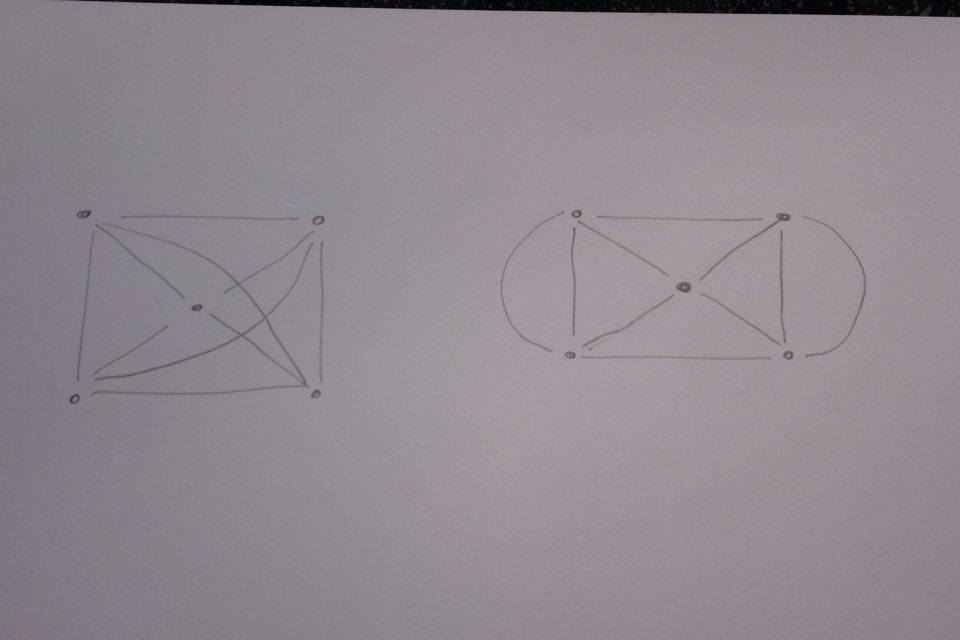
\includegraphics[height=8cm, width=15cm]{gegenbsp.jpg}
\\
\\
Angenommen Graph1, welcher der linke Graph bei der angeführten Abbildung ist, besitzt eine Gradsequenz von $d$ = $(4,4,4,4,4)$ und Graph2, welcher der rechte Graph der Abbildung ist, besitzt ebenfalls eine Gradsequenz von $d$ = $(4,4,4,4,4)$. Man kann nun erkennen, dass bei Graph1 jeder Knoten mit jedem anderen Knoten verbunden ist, somit besitzt dieser einen Durchmesser von 1. Bei Graph2 jedoch kann man erkennen, dass nicht jeder Knoten mit jedem verbunden ist, aber dieser die gleiche Gradsequenz besitzt wie Graph1. Was zur folge hat das Graph 2 einen Durchmesser von 2 besitzt. Somit ist diese Aussage wiederlegt.
\end{document}
